\documentclass{beamer}\usepackage[]{graphicx}\usepackage[]{color}
%% maxwidth is the original width if it is less than linewidth
%% otherwise use linewidth (to make sure the graphics do not exceed the margin)
\makeatletter
\def\maxwidth{ %
  \ifdim\Gin@nat@width>\linewidth
    \linewidth
  \else
    \Gin@nat@width
  \fi
}
\makeatother

\definecolor{fgcolor}{rgb}{0.196, 0.196, 0.196}
\newcommand{\hlnum}[1]{\textcolor[rgb]{0.063,0.58,0.627}{#1}}%
\newcommand{\hlstr}[1]{\textcolor[rgb]{0.063,0.58,0.627}{#1}}%
\newcommand{\hlcom}[1]{\textcolor[rgb]{0.588,0.588,0.588}{#1}}%
\newcommand{\hlopt}[1]{\textcolor[rgb]{0.196,0.196,0.196}{#1}}%
\newcommand{\hlstd}[1]{\textcolor[rgb]{0.196,0.196,0.196}{#1}}%
\newcommand{\hlkwa}[1]{\textcolor[rgb]{0.231,0.416,0.784}{#1}}%
\newcommand{\hlkwb}[1]{\textcolor[rgb]{0.627,0,0.314}{#1}}%
\newcommand{\hlkwc}[1]{\textcolor[rgb]{0,0.631,0.314}{#1}}%
\newcommand{\hlkwd}[1]{\textcolor[rgb]{0.78,0.227,0.412}{#1}}%
\let\hlipl\hlkwb

\usepackage{framed}
\makeatletter
\newenvironment{kframe}{%
 \def\at@end@of@kframe{}%
 \ifinner\ifhmode%
  \def\at@end@of@kframe{\end{minipage}}%
  \begin{minipage}{\columnwidth}%
 \fi\fi%
 \def\FrameCommand##1{\hskip\@totalleftmargin \hskip-\fboxsep
 \colorbox{shadecolor}{##1}\hskip-\fboxsep
     % There is no \\@totalrightmargin, so:
     \hskip-\linewidth \hskip-\@totalleftmargin \hskip\columnwidth}%
 \MakeFramed {\advance\hsize-\width
   \@totalleftmargin\z@ \linewidth\hsize
   \@setminipage}}%
 {\par\unskip\endMakeFramed%
 \at@end@of@kframe}
\makeatother

\definecolor{shadecolor}{rgb}{.97, .97, .97}
\definecolor{messagecolor}{rgb}{0, 0, 0}
\definecolor{warningcolor}{rgb}{1, 0, 1}
\definecolor{errorcolor}{rgb}{1, 0, 0}
\newenvironment{knitrout}{}{} % an empty environment to be redefined in TeX

\usepackage{alltt}

% load packages
\usepackage{tikz}
\usepackage{graphicx}
\usepackage{upquote}
\usepackage{listings}
\usepackage{hyperref}
\usepackage{color}
\usepackage{lmodern}



% define a bunch of colors
\definecolor{gray}{RGB}{110,110,110}
\definecolor{darkgray}{RGB}{100,100,100}
\definecolor{lightgray}{RGB}{200,200,200}
\definecolor{lightgrey}{RGB}{200,200,200}
\definecolor{turquoise}{RGB}{81,193,188}
\definecolor{mamey}{RGB}{255,107,107}
\definecolor{tomato}{RGB}{255,136,136}
\definecolor{mandarina}{RGB}{229,169,25}
\definecolor{lemon}{rgb}{0.81,0.95,0.29}
\definecolor{bluesky}{rgb}{0.71,0.81,0.96}
\definecolor{chiclamino}{RGB}{107,174,214}
\definecolor{violet}{RGB}{133,135,211}

\definecolor{foreground}{RGB}{81,141,193}
\definecolor{background}{RGB}{246,244,240}
\definecolor{highlight}{RGB}{229,169,25}
\definecolor{lowlight}{RGB}{200,200,200}

% setting beamer colors
\setbeamercolor{title}{fg=lightgray}
\setbeamercolor{frametitle}{fg=lightgray}
\setbeamercolor{block title}{fg=turquoise}
\setbeamercolor{structure}{fg=turquoise}
\setbeamercolor{titlelike}{fg=title}
\setbeamercolor{subtitle}{fg=turquoise}
\setbeamercolor{institute}{fg=gray}
\setbeamercolor{normal text}{fg=gray,bg=background}

\setbeamercolor{palette primary}{fg=lightgray}
\setbeamercolor{palette secondary}{fg=lightgray}
\setbeamercolor{palette tertiary}{fg=lightgray}

\setbeamerfont{itemize/enumerate subbody}{size=\footnotesize}
\setbeamerfont{itemize/enumerate subitem}{size=\footnotesize}

\hypersetup{
  colorlinks=true,
  urlcolor=tomato,
  linkcolor=lightgray
}

% commands
\newcommand{\code}[1]{\texttt{#1}}
\newcommand{\high}[1]{\textcolor{highlight}{#1}}
\newcommand{\low}[1]{\textcolor{lowlight}{#1}}
\newcommand{\highcode}[1]{\textcolor{highlight}{\texttt{#1}}}


%\usecolortheme{rose}
\setbeamertemplate{blocks}[rounded]
\setbeamertemplate{footline}[frame number] 
\setbeamertemplate{navigation symbols}{}
\setbeamertemplate{frametitle}[default][center]
\useoutertheme{infolines}  % add footlines
\setbeamersize{text margin left=25pt,text margin right=25pt}



% to remove empty brackets of \institution
\makeatletter
\setbeamertemplate{footline}
{
  \leavevmode%
  \hbox{%
  \begin{beamercolorbox}[wd=.333333\paperwidth,ht=2.25ex,dp=1ex,center]{author in head/foot}%
    \usebeamerfont{author in head/foot}\insertshortauthor%~~\beamer@ifempty{\insertshortinstitute}{}{(\insertshortinstitute)}
  \end{beamercolorbox}%
  \begin{beamercolorbox}[wd=.333333\paperwidth,ht=2.25ex,dp=1ex,center]{title in head/foot}%
    \usebeamerfont{title in head/foot}\insertshorttitle
  \end{beamercolorbox}%
  \begin{beamercolorbox}[wd=.333333\paperwidth,ht=2.25ex,dp=1ex,right]{date in head/foot}%
    \usebeamerfont{date in head/foot}\insertshortdate{}\hspace*{2em}
    \insertframenumber{} / \inserttotalframenumber\hspace*{2ex} 
  \end{beamercolorbox}}%
  \vskip0pt%
}
\makeatother



\title[Getting data from the web with R]{\LARGE Getting Data from the Web with R} 
\subtitle[Web Data in R]{\large Part 8: Getting Data via Web APIs}
\author[gastonsanchez.com]{
 \textcolor{gray}{\textbf{G}aston \textbf{S}anchez}
}
\institute[]{\scriptsize \textcolor{lightgray}{April-May 2014}}
\date[CC BY-SA-NC 4.0]{
 \textcolor{lightgray}{\tiny{Content licensed under 
 \href{http://creativecommons.org/licenses/by-nc-sa/4.0/}{CC BY-NC-SA 4.0}}}
}
\IfFileExists{upquote.sty}{\usepackage{upquote}}{}
\begin{document}




%--- the titlepage frame -------------------------%

\begin{frame}[plain]
 \titlepage
\end{frame}

%------------------------------------------------

{ % all template changes are local to this group.
    \setbeamertemplate{navigation symbols}{}
    \begin{frame}[plain]
        \begin{tikzpicture}[remember picture,overlay]
            \node[at=(current page.center)] {
                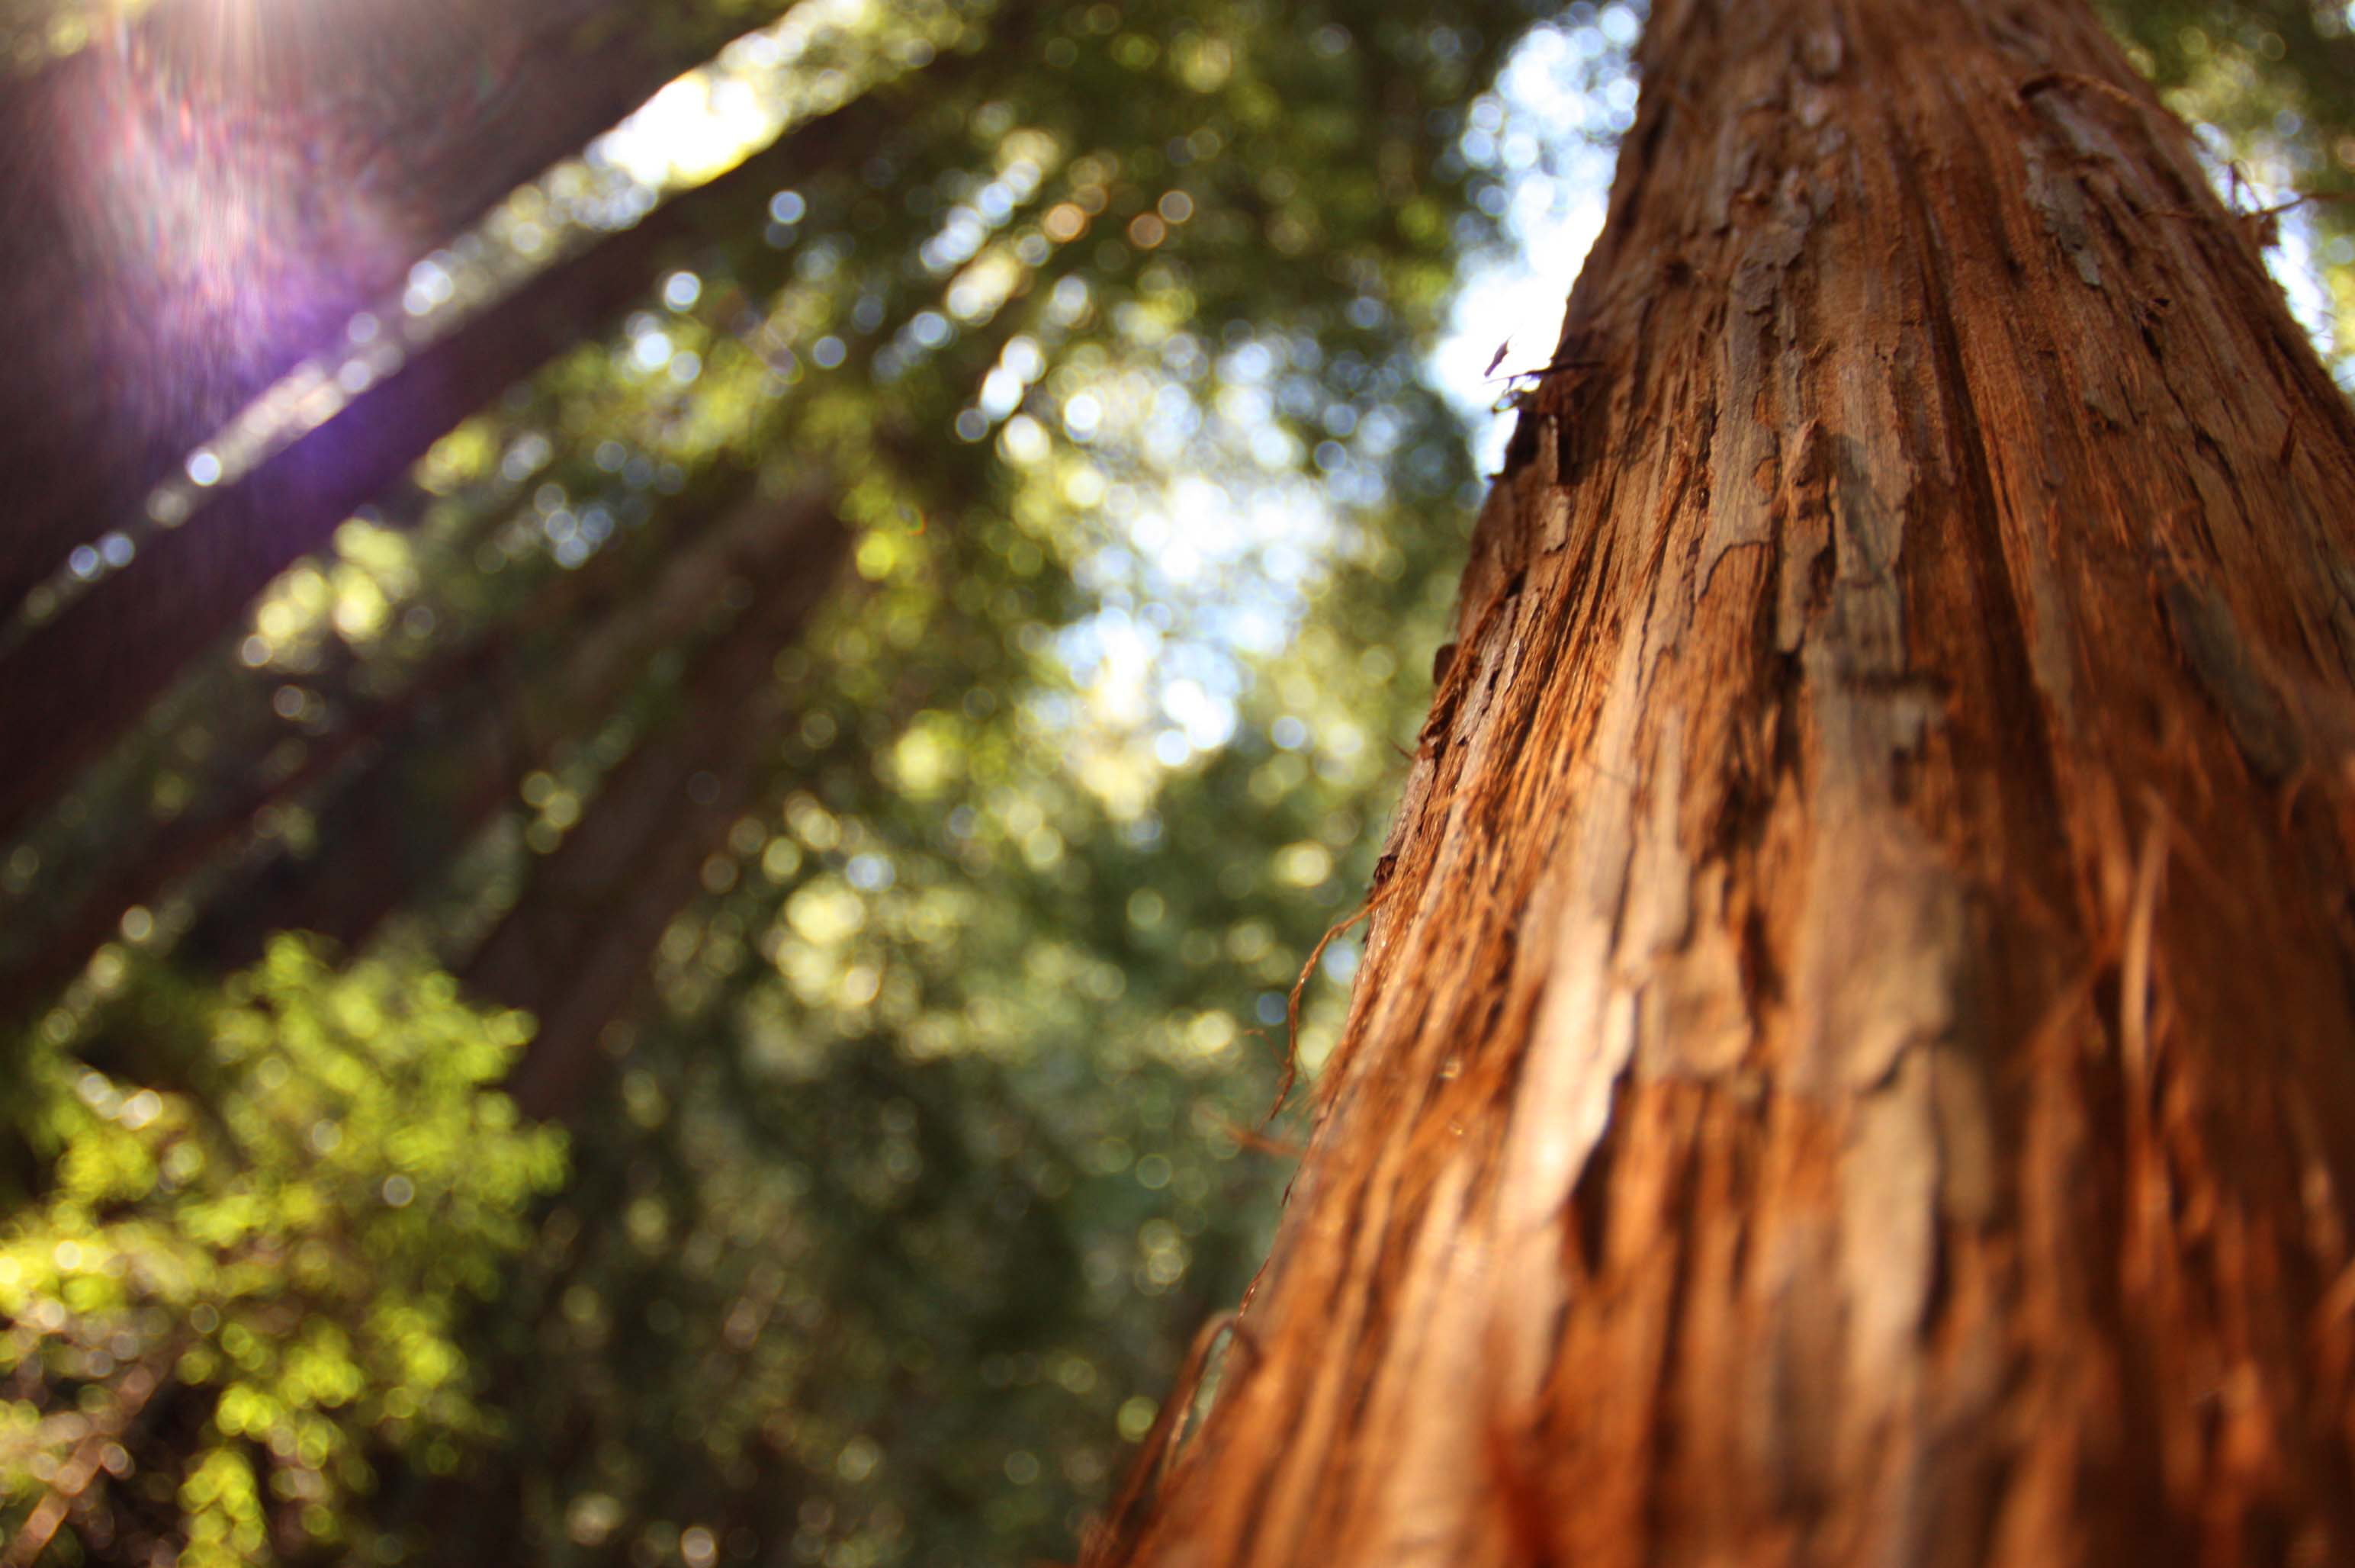
\includegraphics[height=\paperheight]{images/redwood.jpg}
            };
        \end{tikzpicture}
     \end{frame}
}

%------------------------------------------------

\begin{frame}[fragile]
\frametitle{Readme}

\begin{block}{\scriptsize License:}
\tiny
 \begin{itemize}
  \item[] Creative Commons Attribution-NonCommercial-ShareAlike 4.0 International License \\ 
  \url{http://creativecommons.org/licenses/by-nc-sa/4.0/}{}
 \end{itemize}
\end{block}

\begin{block}{\scriptsize You are free to:}
\tiny
 \begin{itemize}
  \item[] \textcolor{darkgray}{\textbf{Share}} --- \textcolor{gray}{copy and redistribute the material}
  \item[] \textcolor{darkgray}{\textbf{Adapt}} --- \textcolor{gray}{rebuild and transform the material}
 \end{itemize}
\end{block}

\vspace{2mm}
\begin{block}{\scriptsize Under the following conditions:}
\tiny
\begin{itemize}
 \item[] \textcolor{darkgray}{\textbf{Attribution}} --- \textcolor{gray}{You must give appropriate credit, provide a link to the license, and indicate if changes were made.}
 \item[] \textcolor{darkgray}{\textbf{NonCommercial}} --- \textcolor{gray}{You may not use this work for commercial purposes.}
 \item[] \textcolor{darkgray}{\textbf{Share Alike}} --- \textcolor{gray}{If you remix, transform, or build upon this 
 work, you must distribute your contributions under the same license to this one.}
\end{itemize}
\end{block}

\end{frame}

%------------------------------------------------

\begin{frame}
\frametitle{Lectures Menu}

\begin{columns}[t]
\begin{column}{0.1\textwidth}
%--- empty space ---%
\end{column}
\begin{column}{0.8\textwidth}
 \begin{block}{Slide Decks}
  \begin{enumerate}
   \item \textcolor{lightgray}{Introduction}
   \item \textcolor{lightgray}{Reading files from the Web}
   \item \textcolor{lightgray}{Basics of XML and HTML}
   \item \textcolor{lightgray}{Parsing XML / HTML content}
   \item \textcolor{lightgray}{Handling JSON data}
   \item \textcolor{lightgray}{HTTP basics and the RCurl package}
   \item \textcolor{lightgray}{Getting data via Web Forms}
   \item \textbf{Getting data via Web APIs}
   %\item \textcolor{lightgray}{Web Scraping Case Study}
  \end{enumerate}
 \end{block}
\end{column}
\begin{column}{0.1\textwidth}
%--- empty space ---%
\end{column}
\end{columns}

\end{frame}

%------------------------------------------------

\begin{frame}
 \begin{center}
  \Huge{\textcolor{mandarina}{Web APIs}}
 \end{center}
\end{frame}

%------------------------------------------------

\begin{frame}
\frametitle{Goal}

\begin{columns}[t]
\begin{column}{0.1\textwidth}
%--- empty space ---%
\end{column}
\begin{column}{0.8\textwidth}

\begin{block}{Data via Web APIs}
The goal of the present slides is to give you an overview of \textbf{how data can be accessed via APIs} with R
\end{block}

\end{column}
\begin{column}{0.1\textwidth}
%--- empty space ---%
\end{column}
\end{columns}

\end{frame}

%------------------------------------------------

\begin{frame}
\frametitle{Synopsis}

\begin{columns}[t]
\begin{column}{0.1\textwidth}
%--- empty space ---%
\end{column}
\begin{column}{0.8\textwidth}

\begin{block}{In a nutshell}
We'll cover the following topics:
\begin{itemize}
 \item API basics
 \item API consederations
 \item Case Study PubMed
\end{itemize}
\end{block}

\end{column}
\begin{column}{0.1\textwidth}
%--- empty space ---%
\end{column}
\end{columns}

\end{frame}

%------------------------------------------------

\begin{frame}
\frametitle{Some References}

\begin{itemize}
 \item XML and Web Technlogies for Data Sciences with R \\
 \low{by Deb Nolan and Duncan Temple Lang}
 \item RESTful Web Services \\
 \low{by Leonard Richardson and Sam Ruby}
 \item The ROAuth Package \\
 {\scriptsize \url{http://cran.r-project.org/web/packages/ROAuth/index.html}}
 \item CRAN Task View: Web Technologies and Services \\
 {\scriptsize \url{http://cran.r-project.org/web/views/WebTechnologies.html}}
\end{itemize}

\end{frame}

%------------------------------------------------

\begin{frame}
 \begin{center}
  \Huge{\textcolor{mandarina}{API Basics}}
 \end{center}
\end{frame}

%------------------------------------------------

\begin{frame}
\frametitle{API}

\begin{quotation}
``In computer programming, an application programming interface (API) specifies how some software components should interact with each other.''
\end{quotation}

\begin{quotation}
``When used in the context of web development, an API is typically defined as a set of Hypertext Transfer Protocol (HTTP) request messages, along with a definition of the structure of response messages''
\end{quotation}

{\scriptsize 
\hspace{8mm} \url{http://en.wikipedia.org/wiki/Application\_programming\_interface}
}

\end{frame}

%------------------------------------------------

\begin{frame}
\frametitle{About APIs}

\begin{block}{What's an API?}
API stands for \textbf{Application Programming Interface}. Broadly speaking, API refers to a set of programming instructions that allow different software to interact with another. 
\end{block}

\begin{block}{Web API?}
A Web API uses HTTP requests to access information from Web-based software application.
\end{block}

\end{frame}

%------------------------------------------------

\begin{frame}
\frametitle{About APIs}

\begin{block}{What's an API?}
By definition, an API is an interface, that is, something that \textbf{defines the way in which two software communicate}.
\end{block}

\begin{block}{How Web APIs communicate?}
With Web APIs, the communication between applications is handled through a collection of standards and protocols \low{(eg HTTP)}
\end{block}

\end{frame}

%------------------------------------------------

\begin{frame}
\frametitle{Importance}

\begin{block}{Why should we care?}
A lot of companies allow users to freely access data from their websites by means of APIs. So it is important to have some exposure on how to work and get data with APIs.
\end{block}

\begin{block}{Everybody who's anybody has an API}
Web APIs are becoming increasingly popular for any company, almost mandatory if they want to stay ``connected'' with the rest of the world, and have a presence with their users/customers. A good starting point for finding more websites with APIs is \textbf{Programmable Web}: \\
{\footnotesize \url{http://www.programmableweb.com}}
\end{block}

\end{frame}

%------------------------------------------------

\begin{frame}
\frametitle{Web API Examples: Google APIs}

\begin{center}
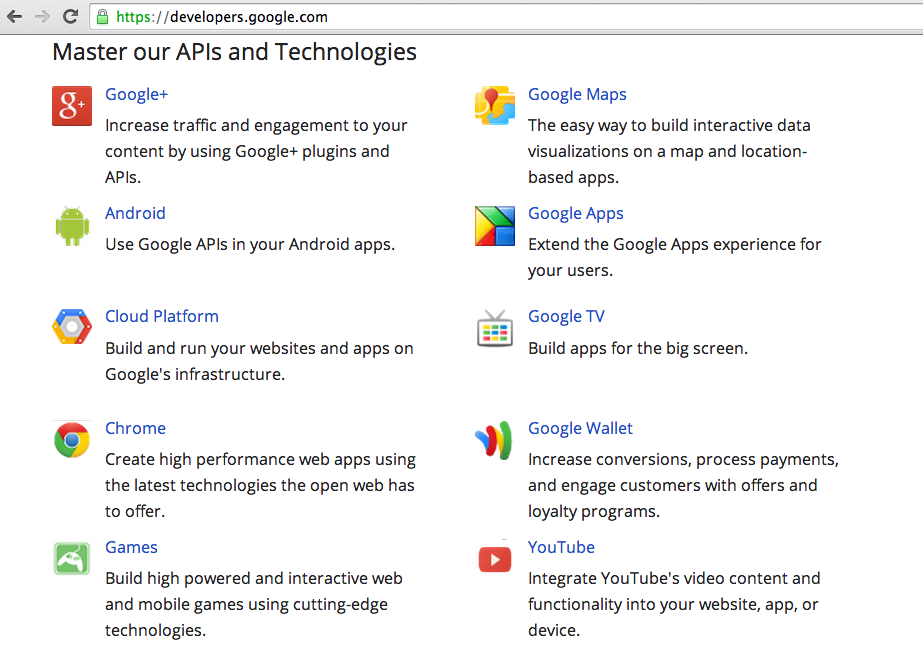
\includegraphics[width=10cm]{images/google_apis.png}
\end{center}

\end{frame}

%------------------------------------------------

\begin{frame}
\frametitle{Web API Examples: Bitly}

\begin{center}
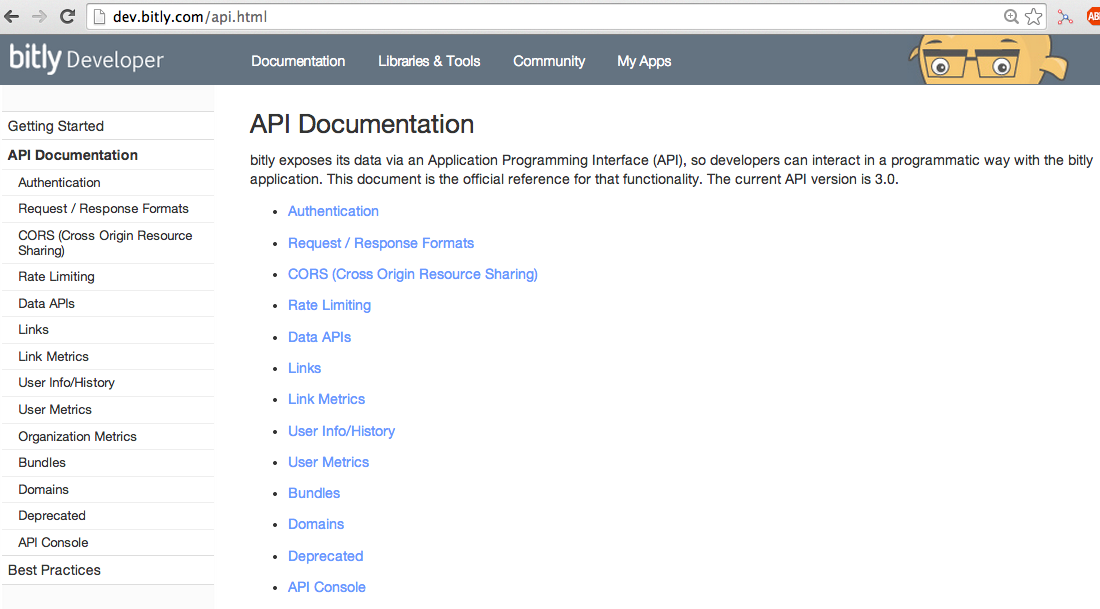
\includegraphics[width=11cm]{images/bitly_api.png}
\end{center}

\end{frame}

%------------------------------------------------

\begin{frame}
\frametitle{Web API Examples: US Census}

\begin{center}
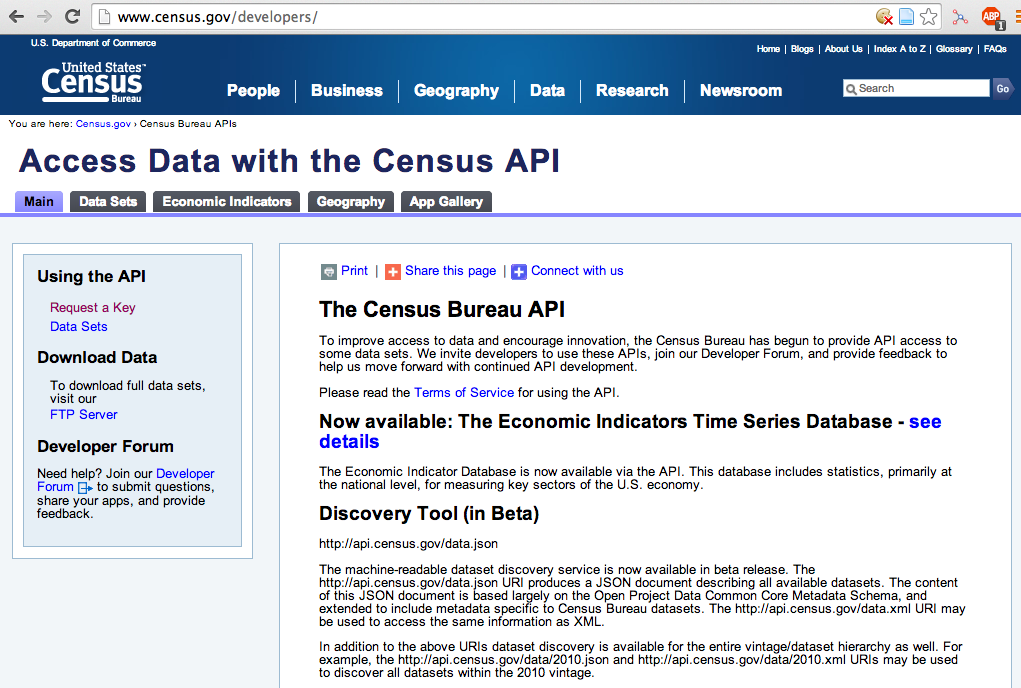
\includegraphics[width=11cm]{images/us_census_api.png}
\end{center}

\end{frame}

%------------------------------------------------

\begin{frame}
 \begin{center}
  {\Huge \textcolor{mandarina}{Web API Considerations}}
 \end{center}
\end{frame}

%------------------------------------------------

\begin{frame}
\frametitle{Considerations}

\begin{columns}[t]
\begin{column}{0.1\textwidth}
%--- empty space ---%
\end{column}
\begin{column}{0.8\textwidth}

\begin{block}{We're just here for the data}
We're interested in Web APIs because they allow us to download content and data. And as with any other tool, there's the good, the bad, and the ugly about Web APIs.
\end{block}

\end{column}
\begin{column}{0.1\textwidth}
%--- empty space ---%
\end{column}
\end{columns}

\end{frame}

%------------------------------------------------

\begin{frame}
\frametitle{Considerations}

\begin{block}{The Good}
\begin{itemize}
 \item Obviously, we get access to data 
 \item No need to buy or pay for data 
 \item We can get access in a programmatically way
 \item There are some R packages for working with specific Web APIs \\
{\scriptsize \url{http://cran.r-project.org/web/views/WebTechnologies.html}}
 \item Under ideal circumnstances, data is in nice formats and decent structure
\end{itemize}
\end{block}

\end{frame}

%------------------------------------------------

\begin{frame}
\frametitle{Considerations}

\begin{block}{The Bad}
\begin{itemize}
 \item You first have to learn how to use a given Web API
 \item Learning about an API and reading the documentation may take you some time
 \item The documentation may be very limited, outdated, and poorly explained
 \item Sometimes the data is not what you were expecting
\end{itemize}
\end{block}

\end{frame}

%------------------------------------------------

\begin{frame}
\frametitle{Considerations}

\begin{block}{The Ugly}
\begin{itemize}
 \item APIs change and evolve, so if you're planning to use one over a long period of time, you have to check it constantly
 \item You may need to register, get credentials, use authentication
 \item Usually there are rate and quota limits on how much data you can download and how frequently
 \item Some APIs can be very complex to use (not user friendly)
\end{itemize}
\end{block}

\end{frame}

%------------------------------------------------

\begin{frame}
\frametitle{Working with Web APis}

\begin{block}{Checklist for working with Web APIs}
\begin{itemize}
 \item Read the API's documentation (check the examples!)
 \item Read terms of service (what you're allowed or not to do)
 \item Typically you may need an API key
 \item You may need to register and open a developer account
 \item You may need to authenticate (just another step in the pipeline)
 \item See what kind of data you have access to
 \item See what kind of formats are available
\end{itemize}
\end{block}

\end{frame}

%------------------------------------------------

\begin{frame}
\frametitle{Working with Web APIs}

\begin{block}{Working with Web APIs and R}
This is our main concern: figure out how to interact with Web APIs and do things in R
\begin{itemize}
 \item Understand how the API works \\
 \low{(eg REST, SOAP)}
 \item Understand what kind of requests you need to use \\
 \low{(GET, POST, etc)}
 \item Experiment first with simple examples
 \item Usually you begin with some kind of query or search
 \item Check what R packages you must load \\
 \low{(eg XML, RCurl, SSOAP, ROAuth, httpRequest, RJSONIO)}
 \item Write functions and scripts (programmatically)
\end{itemize}
\end{block}

\end{frame}

%------------------------------------------------

\begin{frame}
 \begin{center}
  \Huge{\textcolor{mandarina}{Case Study \\ E-utilities with PubMed}}
 \end{center}
\end{frame}

%------------------------------------------------

\begin{frame}
\frametitle{Case Study Outline}

\begin{block}{Outline}
We'll work with a \textbf{small but real life example}, which means you might get lost with all the descriptive information. 

\bigskip
Hopefully this brief outline will help you to navigate through this case study:
\begin{itemize}
 \item \textbf{NCBI} Website
 {\scriptsize \low{(central site containing everything else)}}
 \item Database \textbf{PubMed}
 {\scriptsize \low{(this is where we want to get data from)}}
 \item Web API \textbf{E-Utilities} 
 {\scriptsize \low{(this is the API we'll be playing with)}}
 \item \textbf{ESearch} and \textbf{ESummary}
 {\scriptsize \low{(in particular, we'll use these 2 \textit{functions})}}
\end{itemize}
\end{block}

\end{frame}

%------------------------------------------------

\begin{frame}
\frametitle{National Center for Biotechnology Information}

\begin{center}
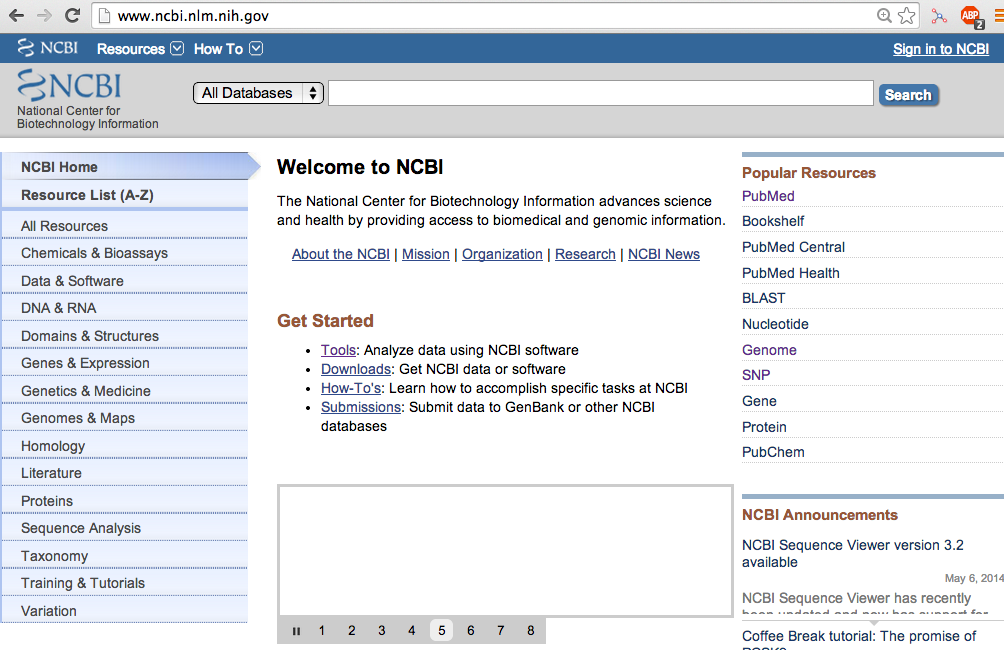
\includegraphics[width=11cm]{images/ncbi_webpage.png}
\end{center}

\end{frame}

%------------------------------------------------

\begin{frame}
\frametitle{About NCBI}

\begin{block}{NCBI}
The \textbf{National Center for Biotechnology Information} (NCBI) provides access to biomedical information \\
{\scriptsize \url{http://www.ncbi.nlm.nih.gov}}
\end{block}

\begin{block}{Mind you}
\begin{itemize}
 \item The NCBI website is kind of ugly and confusing. \\
 \low{(I told you this is a real life example!)}
 \item Looking at the website, it's not evident what you are supposed to do first or where to begin with.
 \item For our example, the important parts of the website are the \textbf{Databases} and the \textbf{Tools}.
\end{itemize}
\end{block}

\end{frame}

%------------------------------------------------

\begin{frame}
\frametitle{About NCBI}

\begin{block}{NCBI Databases}
The real juice of the NCBI website is the data in it. There are \textbf{38 databases} covering a variety of biomedical data. Among them, there is the database \textit{PubMed}.
\end{block}

\begin{center}
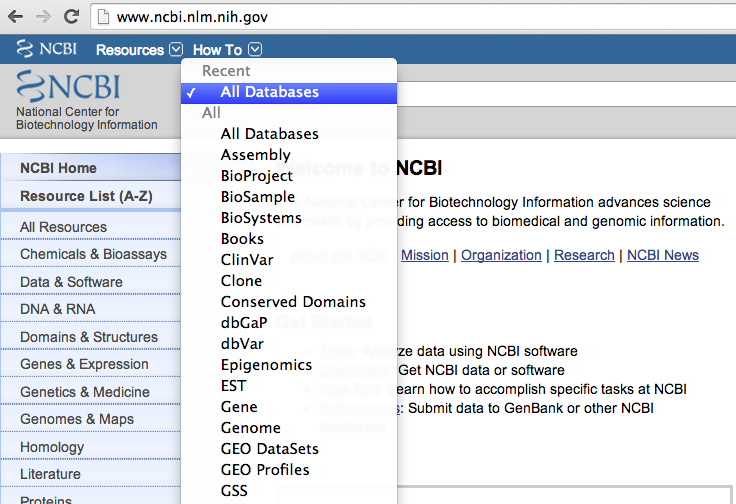
\includegraphics[width=6cm]{images/ncbi_databases.png}
\end{center}

\end{frame}

%------------------------------------------------

\begin{frame}
\frametitle{API: E-Utilities}

\begin{block}{E-Utilities}
The NCBI makes accessible the information in their databases with its API \textbf{Entrez Programming Utilities} also known as \textbf{E-Utilities} \\
{\scriptsize \url{http://www.ncbi.nlm.nih.gov/books/NBK25501/}}
\end{block}

\begin{center}
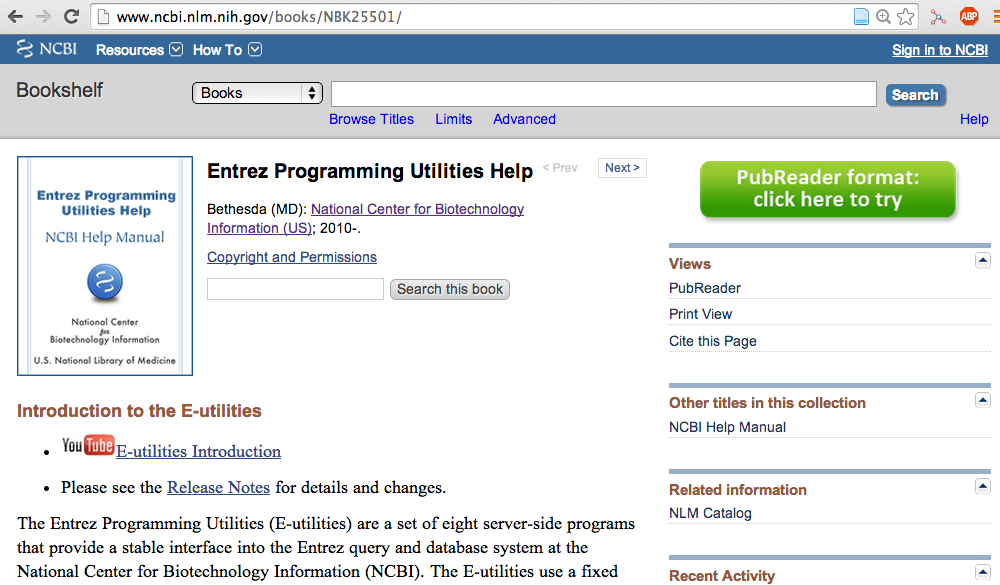
\includegraphics[width=8cm]{images/eutilities_webpage.png}
\end{center}

\end{frame}

%------------------------------------------------

\begin{frame}
\frametitle{About PubMed}

\begin{block}{PubMed Database}
PubMed comprises more than 23 million citations for biomedical literature from MEDLINE, life science journals, and online books. \\
{\scriptsize \url{http://www.ncbi.nlm.nih.gov/pubmed/}}
\end{block}

\begin{center}
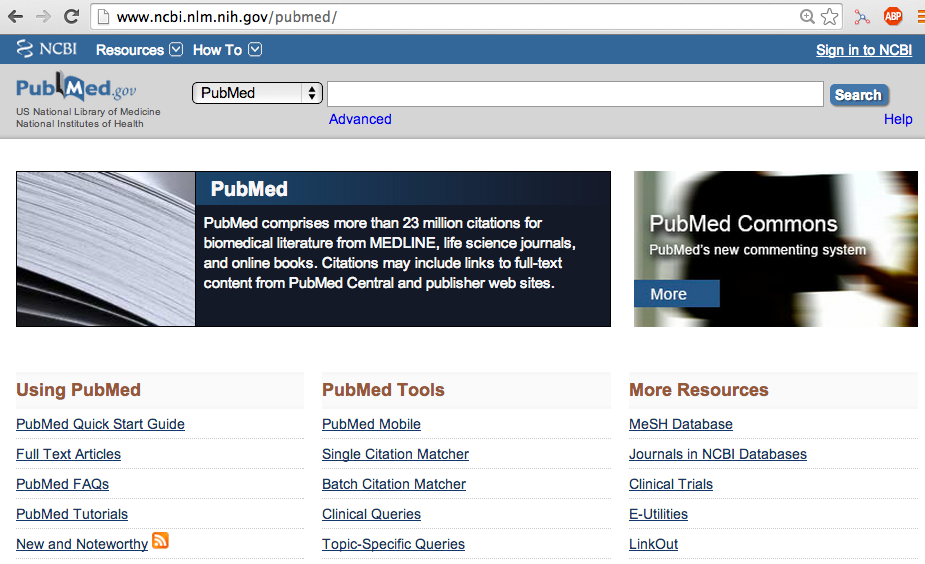
\includegraphics[width=9cm]{images/pubmed_webpage.png}
\end{center}

\end{frame}

%------------------------------------------------

\begin{frame}
\frametitle{Searching PubMed}

Although we can use the Advanced Search forms to query PubMed {\scriptsize (\url{http://www.ncbi.nlm.nih.gov/pubmed/advanced}}), we'll see how to use the E-utilities API to get some data. 

\begin{center}
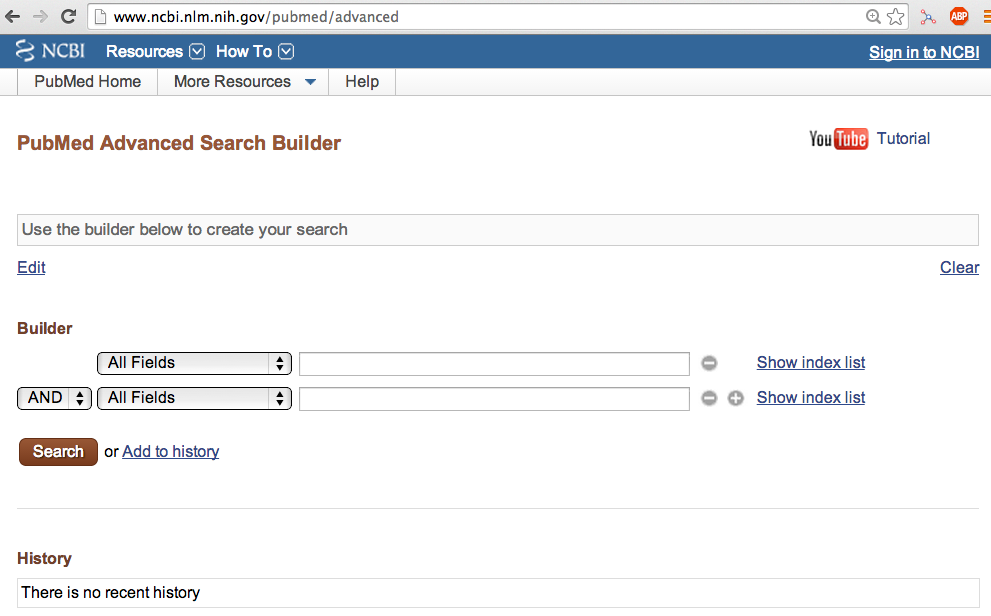
\includegraphics[width=8cm]{images/pubmed_search.png}
\end{center}

\end{frame}

%------------------------------------------------

\begin{frame}
\frametitle{Mission}

\begin{block}{Ultimate Goal}
Your mission is to download the PubMed IDs for articles published in 2012, and containing the term \textit{"human genome"} in their titles 
\end{block}

\begin{center}
\textcolor{turquoise}{Good Luck!}
\end{center}

\end{frame}

%------------------------------------------------

\begin{frame}
 \begin{center}
  {\Huge \textcolor{mandarina}{Basics of E-utilities}}
  
  \vspace{2mm}
  {\Large \textcolor{mandarina}{(NCBI Web API)}}
 \end{center}
\end{frame}

%------------------------------------------------

\begin{frame}
\frametitle{E-Utilities}

E-Utilities provides 8 different applications or utilities:

\begin{center}
 \begin{tabular}{l l}
  \hline
  Application & Description \\
  \hline
  \code{EInfo} & database statistics \\
  \code{ESearch} & text searches \\
  \code{EPost} & Unique Identification (UID) uploads \\
  \code{ESummary} & document summary downloads \\
  \code{EFetch} & data record downloads \\
  \code{ELink} & Entrez links \\
  \code{EGQuery} & global query \\
  \code{ESpell} & spelling suggestions \\
  \code{ECitMatch} & batch citation searching in PubMed \\
  \hline
 \end{tabular}
\end{center}

We'll focus on \textit{ESearch} and \textit{ESummary}

\end{frame}

%------------------------------------------------

\begin{frame}
\frametitle{E-Utilities Documentation}

\begin{block}{Documentation}
Like many other Web APIs, there's an extensive documentation about E-Utilities ... and it's not beginner friendly. 

\bigskip
But this is a good example of the things you will find when working with APIs. Usually you will struggle reading and understanding the provided documentation.
\end{block}

\end{frame}

%------------------------------------------------

\begin{frame}
\frametitle{E-Utilities Applications}

\begin{block}{How does E-utilities work?}
In essence, we use E-utilities by specifying URL's and send requests
\begin{enumerate}
 \item All E-utilities calls share the same URL: \\
 \highcode{http://eutils.ncbi.nlm.nih.gov/entrez/eutils/}
 \item Each E-utility has its own structure and parameters: 
 \begin{itemize}
  \item \highcode{esearch.fcgi?db=<database>\&term=<query>}
  \item \highcode{esummary.fcgi?db=<database>\&id=<uid\_list>}
 \end{itemize}
 \item All E-utilities are appended to the base url: \\
{\tiny 
\highcode{http://eutils.ncbi.nlm.nih.gov/entrez/eutils/esearch.fcgi?db=<database>\&term=<query>}
}
\end{enumerate}
\end{block}

\end{frame}

%------------------------------------------------

\begin{frame}
\frametitle{ESearch and ESummary}

\begin{block}{ESearch \& ESummary 2-step process}
The way you'll work with ESearch and ESummary is using a two-step procedure:
\begin{enumerate}
 \item you \textbf{search for a particular query} in order to get a list of UIDs (unique identification). This is done with \textbf{ESearch}
 \item you use the list of UIDs to get a summary of the resources you are looking for. This is done with \textbf{ESummary} 
\end{enumerate}
\end{block}

\end{frame}

%------------------------------------------------

\begin{frame}
\frametitle{ESearch}

\begin{block}{About ESearch}
ESearch allows us to specify a \textbf{search query on a given database}. An ESearch call has the following structue: \\
\highcode{esearch.fcgi?db=<database>\&term=<query>}
\end{block}

\begin{block}{Parameters}
\begin{itemize}
 \item \highcode{<database>} represents the name of the database
 \item \highcode{<query>} represents the terms forming the query
\end{itemize}
\end{block}

\end{frame}

%------------------------------------------------

\begin{frame}
\frametitle{Defining an ESearch Call}

\begin{block}{Example}
We want to searh \textit{PubMed} and get a list of UIDs for those articles containing the term \textit{human genome} in the title, and that were published in \textit{2012}. 
\end{block}

\begin{block}{Parameters}
database: \highcode{pubmed} \\

query: \highcode{human+genome[title]+AND+2012[pdat]}
\end{block}

\begin{block}{ESearch Call}
{\footnotesize
\highcode{esearch.fcgi?db=pubmed\&term=human+genome[title]+AND+2012[pdat]}
}
\end{block}

\end{frame}

%------------------------------------------------

\begin{frame}[fragile]
\frametitle{ESearch with R}

\begin{knitrout}\tiny
\definecolor{shadecolor}{rgb}{1, 1, 1}\color{fgcolor}\begin{kframe}
\begin{alltt}
\hlcom{# load XML}
\hlkwd{library}\hlstd{(XML)}

\hlcom{# E-utilities base url}
\hlstd{base_url} \hlkwb{=} \hlstr{"http://eutils.ncbi.nlm.nih.gov/entrez/eutils/"}

\hlcom{# define database variable: PubMed}
\hlstd{db} \hlkwb{=} \hlstr{"pubmed"}

\hlcom{# define query variable}
\hlstd{query} \hlkwb{=} \hlstr{"human+genome[title]+AND+2012[pdat]"}

\hlcom{# assemble ESearch call}
\hlstd{esearch} \hlkwb{=} \hlkwd{sprintf}\hlstd{(}\hlstr{"esearch.fcgi?db=%s&term=%s"}\hlstd{, db, query)}

\hlcom{# create URL to make search request}
\hlstd{search_url} \hlkwb{=} \hlkwd{paste}\hlstd{(base_url, esearch,} \hlkwc{sep} \hlstd{=} \hlstr{''}\hlstd{)}

\hlcom{# ESearch request to get the list of UIDs}
\hlcom{# (the list will be contained in an XML document)}
\hlstd{search_doc} \hlkwb{=} \hlkwd{xmlParse}\hlstd{(search_url)}
\end{alltt}
\end{kframe}
\end{knitrout}

\end{frame}

%------------------------------------------------

\begin{frame}[fragile]
\frametitle{ESearch XML file output}

{\scriptsize
\begin{verbatim}
<?xml version="1.0" ?>
<!DOCTYPE eSearchResult PUBLIC ...>
<eSearchResult>
  <Count>103</Count>
  <RetMax>20</RetMax>
  <RetStart>0</RetStart>
  <QueryKey>1</QueryKey>
  <WebEnv>NCID_1_282865897_130.14.18.34_9001_1399488846_694838780</WebEnv>
  <IdList>
    <Id>23959643</Id>
    <Id>23730202</Id>
    ...
  </IdList>
   ...
</eSearchResult>
\end{verbatim}
}

There's a \highcode{Count} of 103 articles. Each article has its corresponding \highcode{Id}. By default (\highcode{RetMax}) just 20 \code{Id}s are retrieved
\end{frame}

%------------------------------------------------

\begin{frame}[fragile]
\frametitle{ESearch with R}



In order to get the 103 articles, we need to change the default maximum number of retrieved results:

\begin{knitrout}\tiny
\definecolor{shadecolor}{rgb}{1, 1, 1}\color{fgcolor}\begin{kframe}
\begin{alltt}
\hlcom{# let's add the retmax parameter}
\hlstd{retmax} \hlkwb{=} \hlnum{200}

\hlcom{# redefine assemble ESearch}
\hlstd{new_esearch} \hlkwb{=} \hlkwd{sprintf}\hlstd{(}\hlstr{"esearch.fcgi?db=%s&term=%s&retmax=%s"}\hlstd{, db, query, retmax)}

\hlcom{# update URL to make request}
\hlstd{new_search_url} \hlkwb{=} \hlkwd{paste}\hlstd{(base_url, new_esearch,} \hlkwc{sep} \hlstd{=} \hlstr{''}\hlstd{)}

\hlcom{# ESearch request to get the list of UIDs}
\hlcom{# (the list will be contained in an XML document)}
\hlstd{new_search_doc} \hlkwb{=} \hlkwd{xmlParse}\hlstd{(new_search_url)}
\end{alltt}
\end{kframe}
\end{knitrout}

\end{frame}

%------------------------------------------------

\begin{frame}[fragile]
\frametitle{ESearch with R}



We need to get the list of \highcode{<Id>}'s that are in the XML node \highcode{<IdList>}. One way to get those values is by using \code{xpathSApply()}

\begin{knitrout}\tiny
\definecolor{shadecolor}{rgb}{1, 1, 1}\color{fgcolor}\begin{kframe}
\begin{alltt}
\hlcom{# get UIDs in a vector}
\hlstd{ids} \hlkwb{=} \hlkwd{xpathSApply}\hlstd{(new_search_doc,} \hlkwc{path} \hlstd{=} \hlstr{"//IdList/Id"}\hlstd{,} \hlkwc{fun} \hlstd{=} \hlstr{'xmlValue'}\hlstd{)}

\hlcom{# we should have 103 IDs}
\hlkwd{length}\hlstd{(ids)}
\end{alltt}
\begin{verbatim}
## [1] 103
\end{verbatim}
\begin{alltt}
\hlcom{# take a peek}
\hlkwd{head}\hlstd{(ids)}
\end{alltt}
\begin{verbatim}
## [1] "23959643" "23730202" "23520917" "23281708" "23281599" "23266811"
\end{verbatim}
\begin{alltt}
\hlkwd{tail}\hlstd{(ids)}
\end{alltt}
\begin{verbatim}
## [1] "22057813" "22057783" "22050290" "22031941" "21945885" "21559844"
\end{verbatim}
\end{kframe}
\end{knitrout}

\end{frame}

%------------------------------------------------

\begin{frame}
\frametitle{ESummary}

\begin{block}{About ESummary}
ESummary allows us to get \textit{document summaries} for a list of input UIDs. An ESummary call has the following structure: \\
\highcode{esummary.fcgi?db=<database>\&id=<uid\_list>}
\end{block}

\begin{block}{Parameters}
\begin{itemize}
 \item \highcode{<database>} represents the name of the database
 \item \highcode{<uid\_list>} represents the list of UIDs
\end{itemize}
\end{block}

\end{frame}

%------------------------------------------------

\begin{frame}
\frametitle{ESummary}

\begin{block}{Example}
With ESearch we retrieve the list of UIDs for the articles we're looking for. Now we need to pass the list to ESummary
\end{block}

\begin{block}{Parameters}
database: \highcode{pubmed} \\

uid\_list: \highcode{23959643,23730202,23520917,...}
\end{block}

\begin{block}{ESummary Call}
{\footnotesize
\highcode{esummary.fcgi?db=pubmed\&id=23959643,23730202,23520917,...}
}
\end{block}

\end{frame}

%------------------------------------------------

\begin{frame}[fragile]
\frametitle{ESummary with R}

Now we need to use ESummary to get summaries of each article:

\begin{knitrout}\tiny
\definecolor{shadecolor}{rgb}{1, 1, 1}\color{fgcolor}\begin{kframe}
\begin{alltt}
\hlcom{# concatenate all IDs, separated by commas}
\hlcom{# (we'll pass this list to ESummary)}
\hlstd{id_list} \hlkwb{=} \hlkwd{paste}\hlstd{(ids,} \hlkwc{collapse} \hlstd{=} \hlstr{','}\hlstd{)}

\hlcom{# assemble ESummary call}
\hlstd{esummary} \hlkwb{=} \hlkwd{sprintf}\hlstd{(}\hlstr{"esummary.fcgi?db=%s&id=%s"}\hlstd{, db, id_list)}

\hlcom{# create URL to make request}
\hlstd{sum_url} \hlkwb{=} \hlkwd{paste}\hlstd{(base_url, esummary,} \hlkwc{sep} \hlstd{=} \hlstr{''}\hlstd{)}

\hlcom{# ESummary request to get document summaries}
\hlcom{# (the summaries will be contained in an XML document)}
\hlstd{summary_doc} \hlkwb{=} \hlkwd{xmlParse}\hlstd{(sum_url)}
\end{alltt}
\end{kframe}
\end{knitrout}

\end{frame}

%------------------------------------------------

\begin{frame}[fragile]
\frametitle{ESummary output}

You should get something like this from ESummary:

\begin{knitrout}\tiny
\definecolor{shadecolor}{rgb}{1, 1, 1}\color{fgcolor}\begin{kframe}
\begin{verbatim}
## <?xml version="1.0" encoding="UTF-8"?> 
## <!DOCTYPE eSummaryResult PUBLIC "-//NLM//DTD esummary v1 20060131//EN" "http://eutils.ncbi.nlm.nih.gov/eutils/dtd/20060131/esummary-v1.dtd"> 
## <eSummaryResult> 
## <DocSum> 
## 	<Id>23959643</Id> 
## 	<Item Name="PubDate" Type="Date">2012 Dec</Item> 
## 	<Item Name="EPubDate" Type="Date"></Item> 
## 	<Item Name="Source" Type="String">Hum Biol</Item> 
## 	<Item Name="AuthorList" Type="List"> 
## 		<Item Name="Author" Type="String">Casto AM</Item> 
## 		<Item Name="Author" Type="String">Henn BM</Item> 
## 		<Item Name="Author" Type="String">Kidd JM</Item> 
## 		<Item Name="Author" Type="String">Bustamante CD</Item> 
## 		<Item Name="Author" Type="String">Feldman MW</Item> 
## 	</Item> 
## 	<Item Name="LastAuthor" Type="String">Feldman MW</Item> 
## 	<Item Name="Title" Type="String">A tale of two haplotypes: the EDA2R/AR Intergenic region is the most divergent genomic segment between Africans and East Asians in the human genome.</Item> 
## 	<Item Name="Volume" Type="String">84</Item> 
## 	<Item Name="Issue" Type="String">6</Item> 
## 	<Item Name="Pages" Type="String">641-94</Item> 
## 	<Item Name="LangList" Type="List"> 
## 		<Item Name="Lang" Type="String">English</Item> 
## 	</Item> 
## 	<Item Name="NlmUniqueID" Type="String">0116717</Item> 
## 	<Item Name="ISSN" Type="String">0018-7143</Item>
\end{verbatim}
\end{kframe}
\end{knitrout}

\end{frame}

%------------------------------------------------

\begin{frame}
\frametitle{Journal Names}

The summary document of each \highcode{<Id>} article is composed of several \highcode{<Item>}'s such as \code{"PubDate"}, \code{"AuthorList"}, \code{"Title"}, \code{"Lang"}, and \code{"FullJournalName"}, among others. 

\bigskip
The \textbf{journal name} of each article is in an element: \\
\code{<Item Name="FullJournalName" Type="String">}

\bigskip
For instance, the first article of the list (\code{<Id>23959643</Id>}) was published in \textit{Human Biology}: \\ 
\highcode{<Item Name="FullJournalName" Type="String">Human biology</Item>}

\end{frame}

%------------------------------------------------

\begin{frame}[fragile]
\frametitle{ESummary with R}
If we want to get the journal names in which each article was published, we can use \code{xpathSApply()} like so:



\begin{knitrout}\tiny
\definecolor{shadecolor}{rgb}{1, 1, 1}\color{fgcolor}\begin{kframe}
\begin{alltt}
\hlcom{# journal names}
\hlstd{journals} \hlkwb{=} \hlkwd{xpathSApply}\hlstd{(summary_doc,} \hlstr{"//Item[@Name='FullJournalName']"}\hlstd{, xmlValue)}

\hlcom{# first 5 journals}
\hlkwd{head}\hlstd{(journals,} \hlkwc{n} \hlstd{=} \hlnum{5}\hlstd{)}
\end{alltt}
\begin{verbatim}
## [1] "Human biology"                                                                                                                                      
## [2] "Current genomics"                                                                                                                                   
## [3] "Revista de derecho y genoma humano = Law and the human genome review / Catedra de Derecho y Genoma Humano/Fundacion BBV-Diputacion Foral de Bizkaia"
## [4] "BMC genomics"                                                                                                                                       
## [5] "BMC genomics"
\end{verbatim}
\begin{alltt}
\hlcom{# last 5 journals}
\hlkwd{tail}\hlstd{(journals,} \hlkwc{n} \hlstd{=} \hlnum{5}\hlstd{)}
\end{alltt}
\begin{verbatim}
## [1] "Human genetics"             "Tissue antigens"           
## [3] "Journal of virology"        "Human molecular genetics"  
## [5] "Journal of medical systems"
\end{verbatim}
\end{kframe}
\end{knitrout}

\end{frame}

%------------------------------------------------

\end{document}
